\begin{frame}
\begin{quotation}
{\it One [...] idea, which underlies everything in this book, is the concept
of genomically encoded information processing. [...],
this is like the geological basis of the landscape. In my view, cis-regulatory information processing, and information processing at the gene regulatory network circuit level, are the real secret of animal development. Probably the appearance of genomic regulatory systems capable of information processing is what made animal evolution possible.} -Eric H. Davidson \cite{Davidson2006a}
\end{quotation}
\end{frame}

\begin{frame}
\begin{figure}
\noindent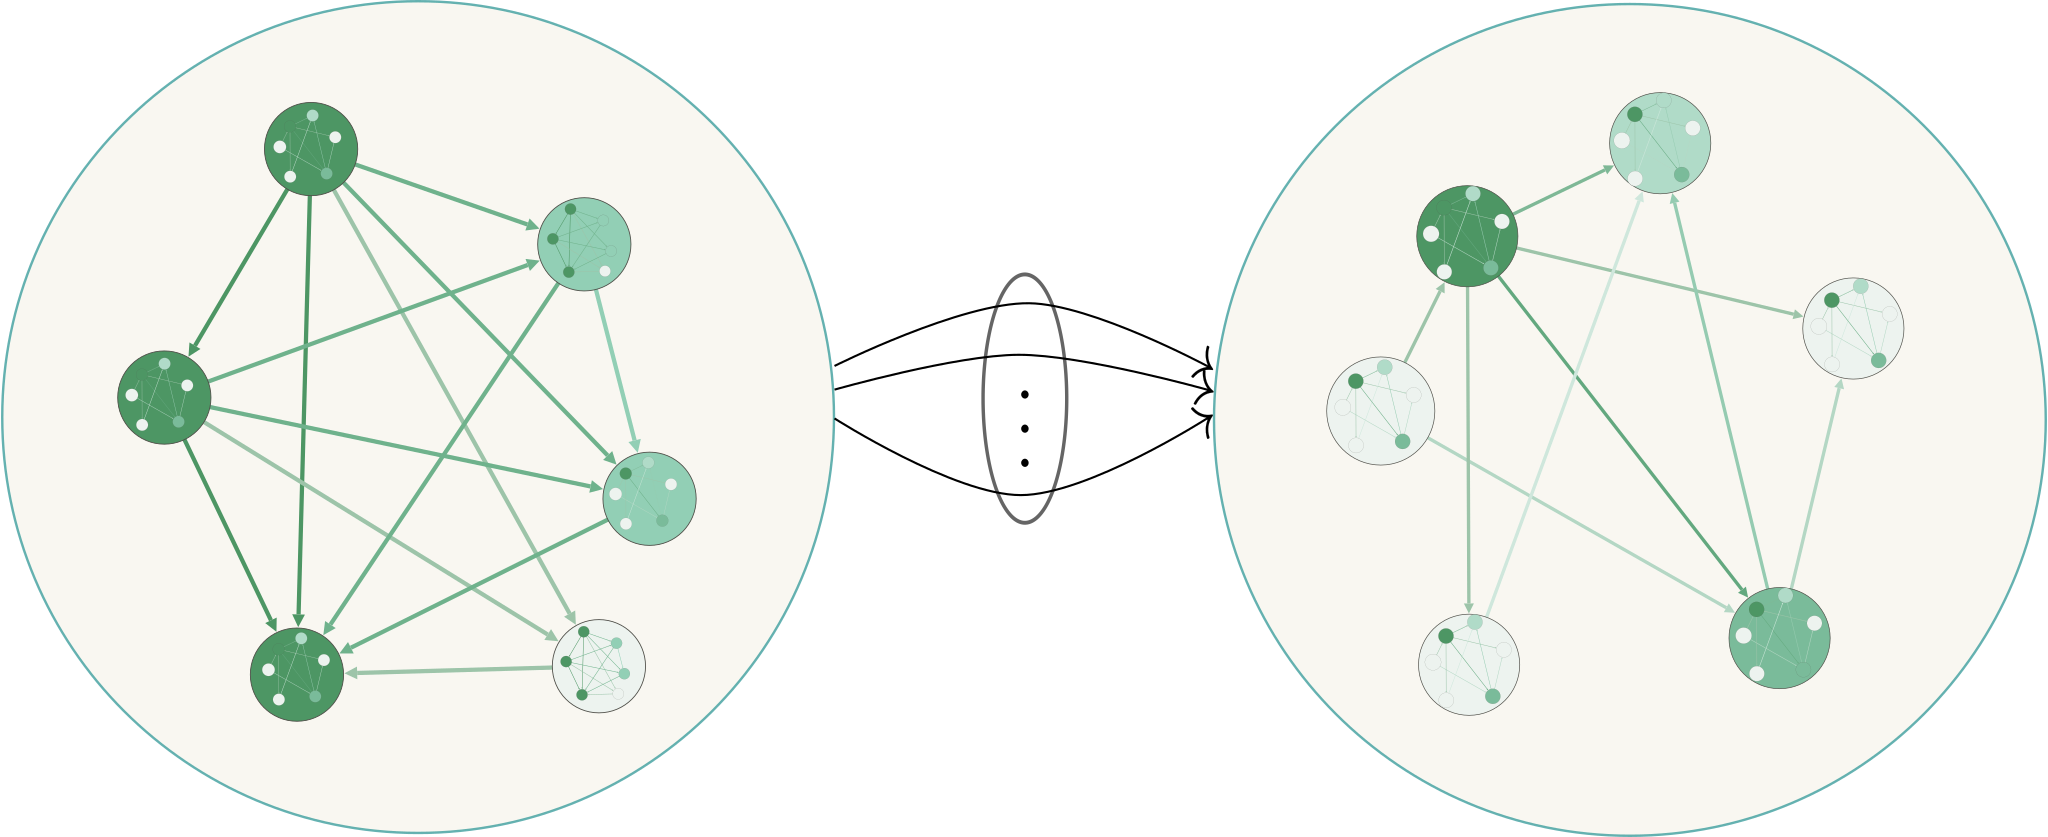
\includegraphics[width=1.0\framewidth]{fig/biograph.pdf}
\caption{%Particular features of interaction networks underlying biological systems can be abstracted as algebraic structures of some type with morphisms translating structure between them. 
On the left is a representation of the integrated metabolic-gene regulatory glycolytic network of E. coli K12 MG1655 derived from the EcoCyc database \cite{Keseler2011} in terms of the BioPAX ontology \cite{Demir2010}. 
%On the right is a conceptual picture of the way in which the relationships between substructure of a particular network can be represented algebraically in terms of algebraic structures that can be referred to as objects and methods of transforming or mapping between these structures referred to as morphisms.}
}
\label{fig:biograph}
\end{figure}
\end{frame}